\begin{figure}[p]\centering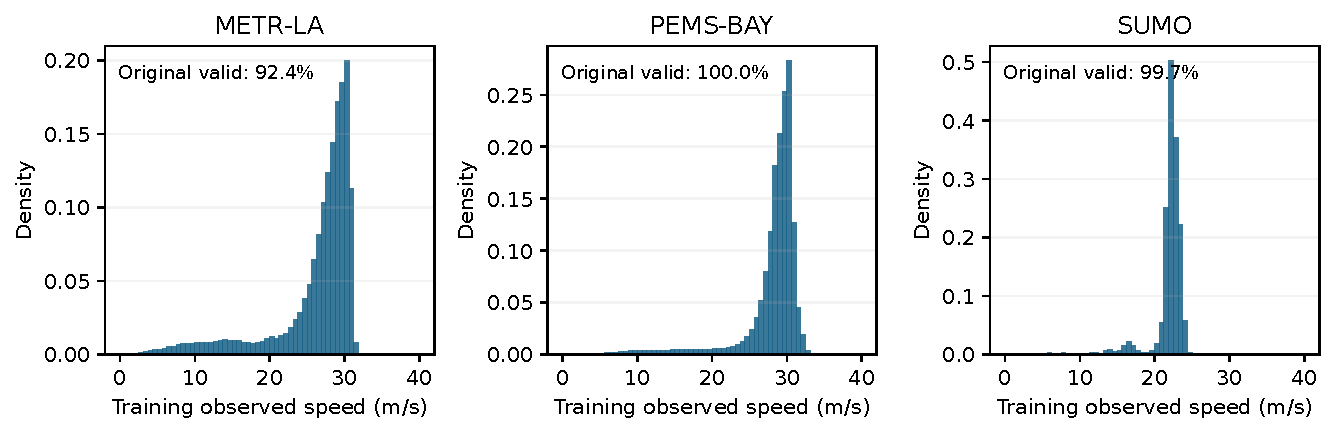
\includegraphics[width=\linewidth]{figures/data-profile.pdf}\caption{Training-partition observed-speed distributions before forecast-window construction. Only originally valid prepared measurements are plotted; labels report original valid fractions. SUMO includes its prepared training-partition measurements. The distributions are descriptive, not an explanation of calibration transfer.}\label{fig:data-profile}\end{figure}\clearpage
\begin{figure}[p]\centering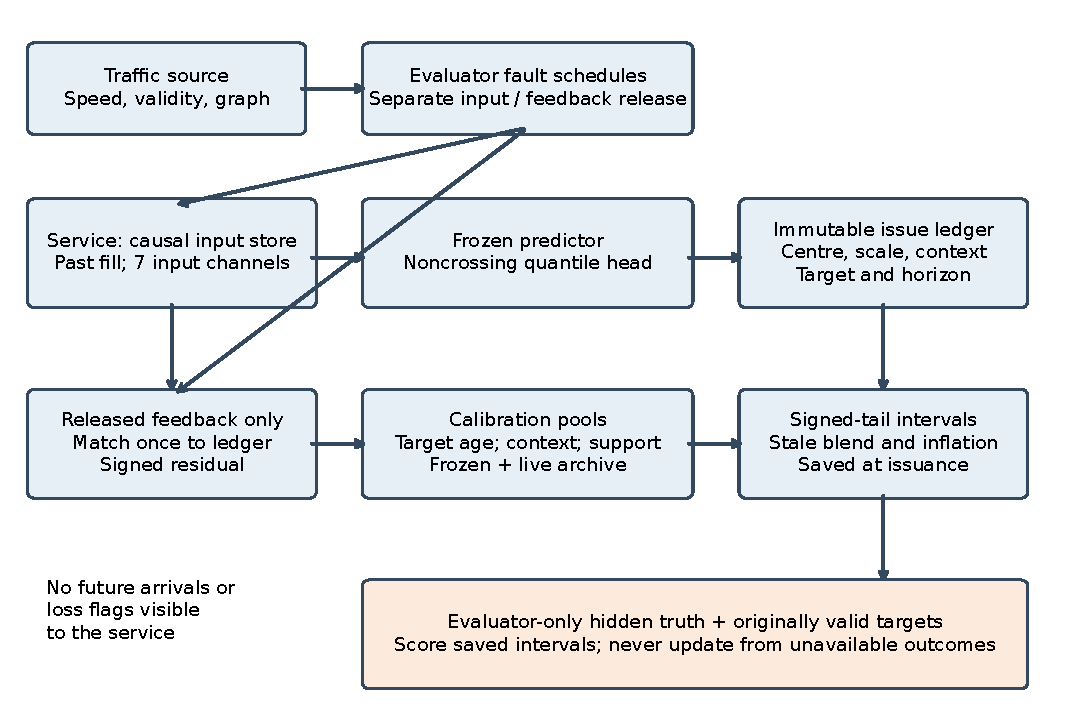
\includegraphics[width=\linewidth]{figures/architecture.pdf}\caption{Causal architecture with separate input, feedback and evaluator lanes. Stored issue records feed both residual matching and the calibration query; the junction is intentional. Hidden truth feeds scoring only. All module routes avoid text and preserve the service information boundary.}\label{fig:architecture}\end{figure}\clearpage
\begin{figure}[p]\centering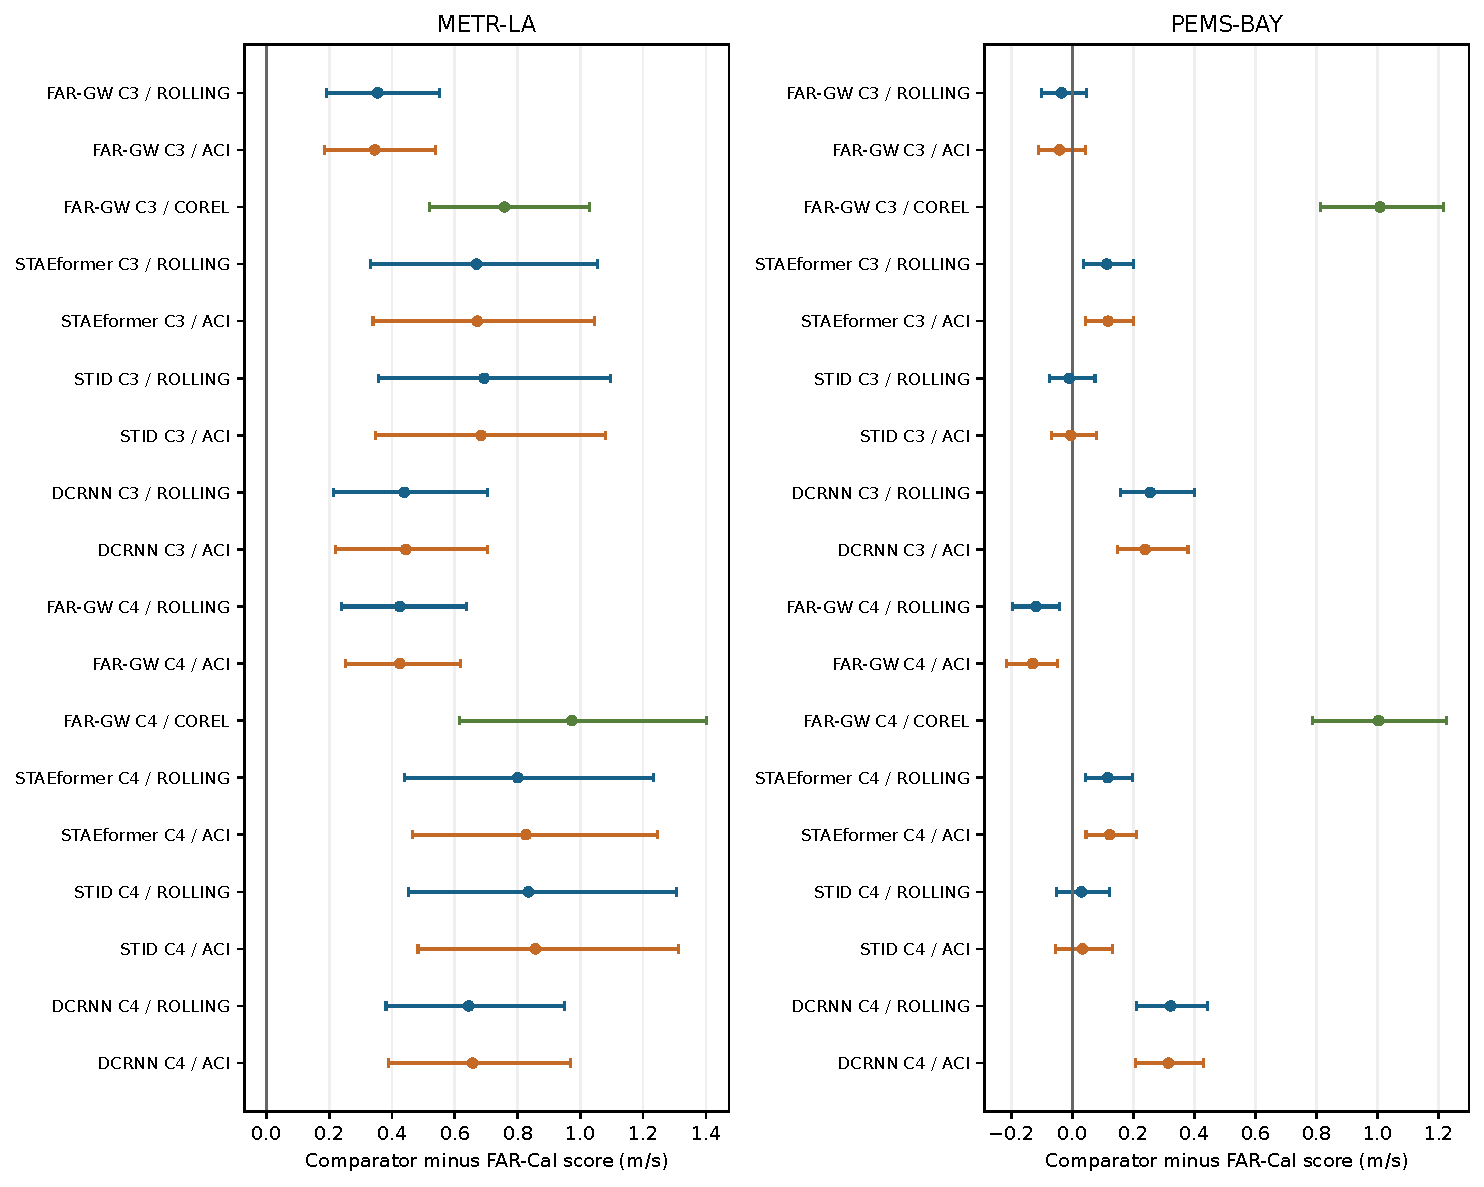
\includegraphics[width=\linewidth]{figures/benchmarks.pdf}\caption{Paired comparator-minus-FAR-Cal interval-score effects and 95\% intervals in SI units. Positive values favour FAR-Cal. Comparisons share frozen forecasts within each backbone; CoRel is restricted to FAR-GW.}\label{fig:benchmarks}\end{figure}\clearpage
\begin{figure}[p]\centering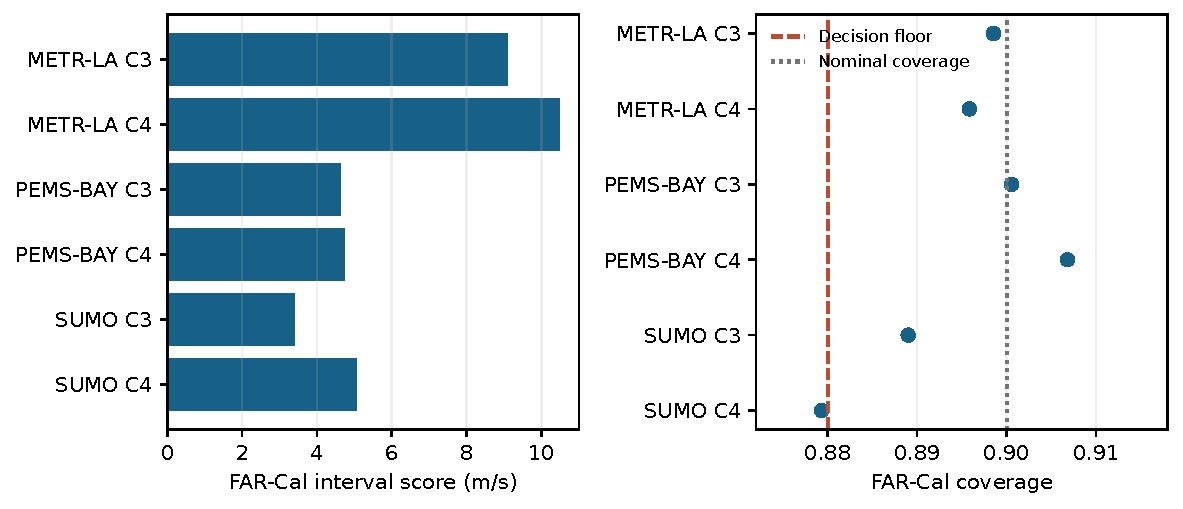
\includegraphics[width=\linewidth]{figures/quality.pdf}\caption{Final FAR-GW interval score and coverage for the six primary cells. Dashed and dotted lines mark the 0.88 decision floor and 0.90 nominal coverage. Absolute network scores are not a paired between-network effect.}\label{fig:quality}\end{figure}\clearpage
\begin{figure}[p]\centering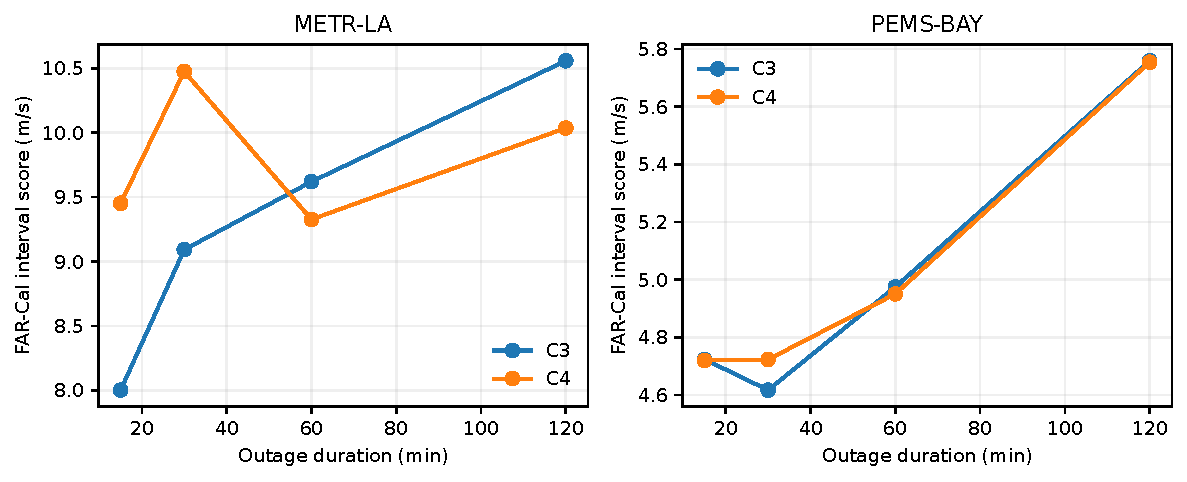
\includegraphics[width=\linewidth]{figures/duration.pdf}\caption{Interval score across the registered outage-duration grid. Lines connect descriptive scores, not interpolation guarantees; C3 and C4 are distinct feedback conditions.}\label{fig:duration}\end{figure}\clearpage
\begin{figure}[p]\centering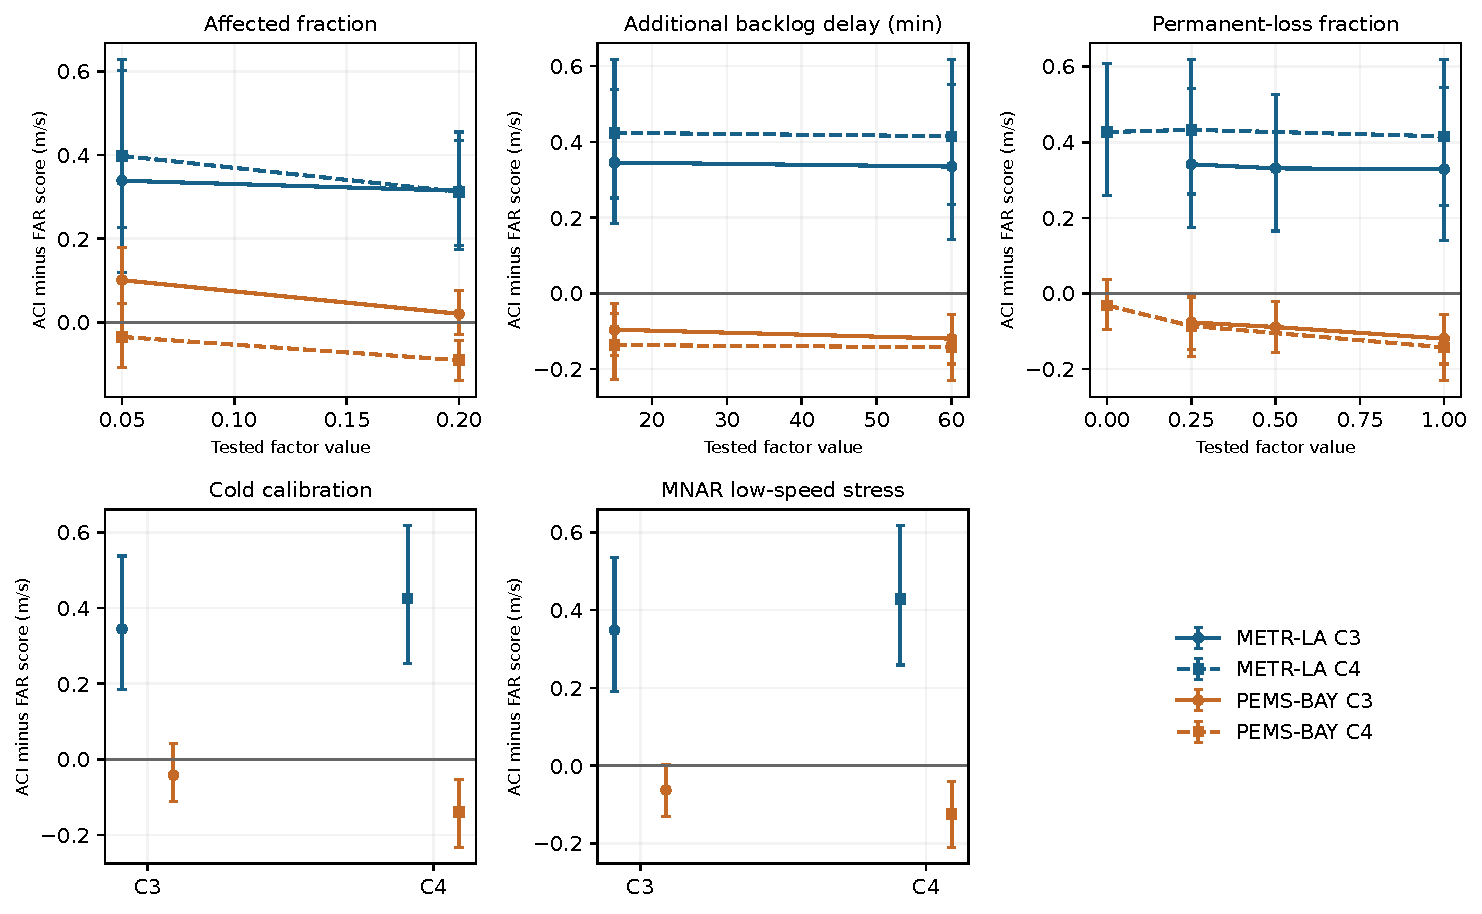
\includegraphics[width=\linewidth]{figures/stress.pdf}\caption{Additional one-factor stress: ACI-minus-FAR-Cal effects and paired 95\% intervals for affected fraction, backlog delay, permanent loss, cold calibration and MNAR. Positive values favour FAR-Cal. Categorical panels contain only their registered conditions; continuous lines connect tested values without extrapolation.}\label{fig:stress}\end{figure}\clearpage
\begin{figure}[p]\centering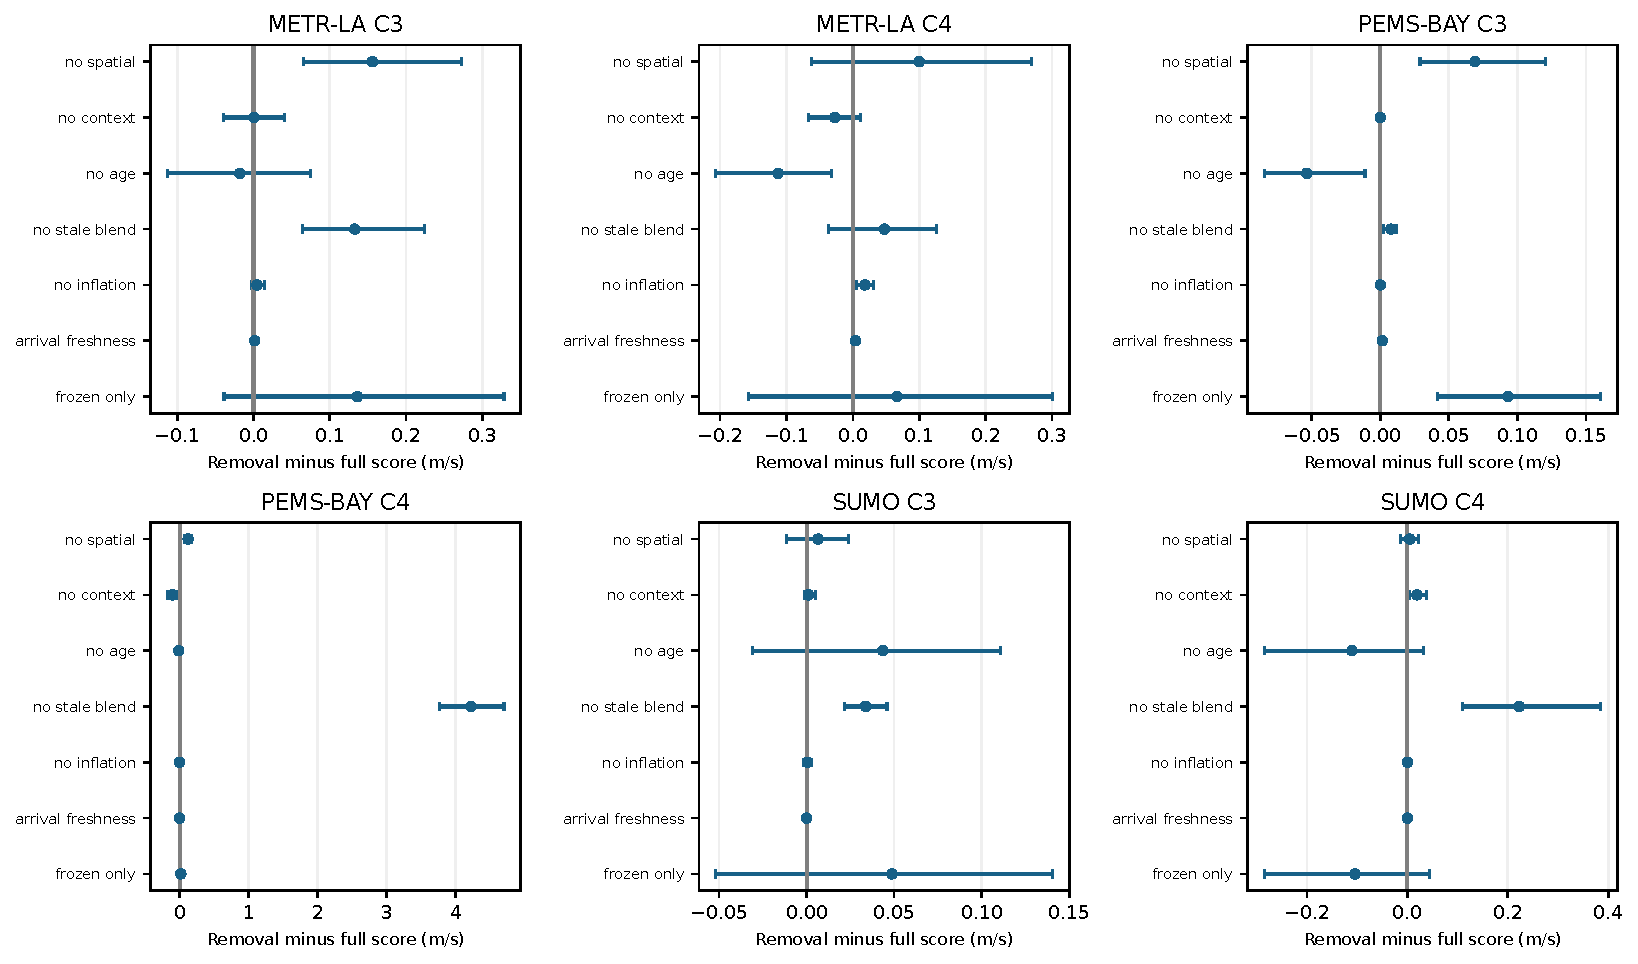
\includegraphics[width=\linewidth]{figures/ablations.pdf}\caption{Exploratory removal-minus-full interval-score effects and 95\% paired intervals. Positive values indicate deterioration after removal. Panel scales differ; the off-scale PEMS-BAY C4 stale-blend failure is explicitly labelled with its estimate and bounds.}\label{fig:ablations}\end{figure}\clearpage
\begin{figure}[p]\centering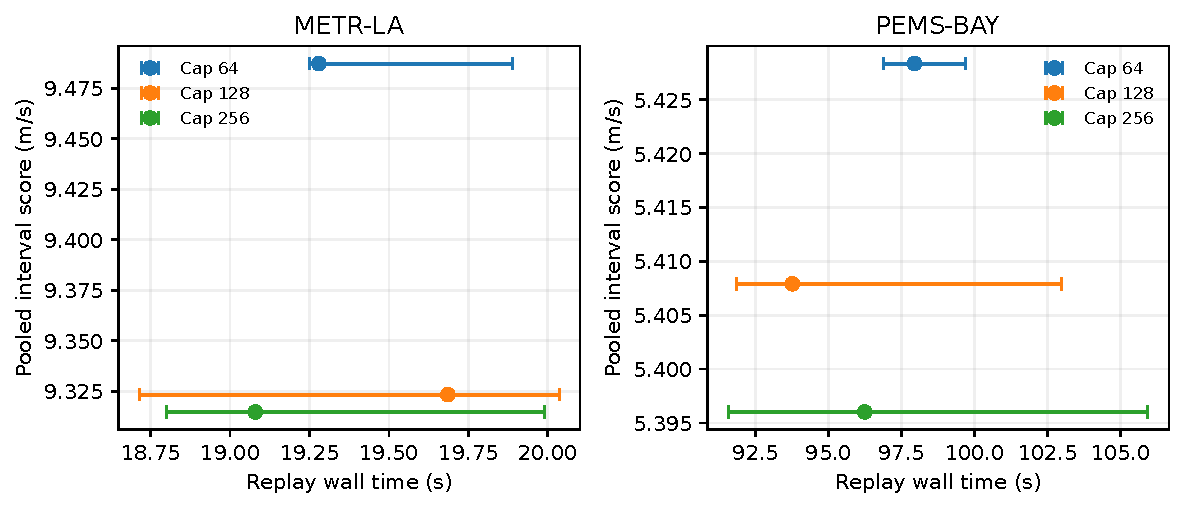
\includegraphics[width=\linewidth]{figures/compute.pdf}\caption{Descriptive archive-cap quality and wall-time sensitivity, with three observed runtime repetitions per cap and network. Horizontal bars are observed ranges, not confidence intervals. These fixed-run pooled scores differ from the origin-level paired inference estimand.}\label{fig:compute}\end{figure}\clearpage